\section{Metodologia}
\subsection{Área de estudo e dados}
\label{sec:dados}

Mato Grosso reúne Amazônia, Cerrado e Pantanal, com diferenças ambientais e trajetórias de ocupação que participam das possibilidades agrícolas. A análise utiliza os 141 municípios da malha de 2023 do Instituto Brasileiro de Geografia e Estatística (IBGE) entre 2001 e 2024. Boa Esperança do Norte não constitui unidade autônoma nessa grade. O bioma de maior fração municipal organiza a comparação territorial, preservando-se as frações dos demais biomas. Há 63 municípios mistos, e a classificação predominante não localiza cada conversão dentro de um bioma nem representa regra uniforme para todos os imóveis.

O percurso descritivo distingue a abertura observada dos incentivos e das condições locais que podem acompanhá-la. As séries de conversão e preços situam as mudanças ao longo do período; a distribuição do potencial caracteriza diferenças persistentes entre municípios; e o desempenho anterior permite reconhecer perdas em relação ao histórico de cada cultura. A cobertura dessas medidas também importa, pois a exigência de histórico altera o conjunto de localidades sobre o qual as hipóteses podem ser examinadas.

A produção e as áreas plantada e colhida provêm da Produção Agrícola Municipal (PAM), e as transições anuais de uso da terra, do MapBiomas Coleção 10.1 \cite{IBGEPAM2026,MapBiomas2026}. A grade contém 3.384 pares município--ano potenciais, dos quais 2.772, em 137 municípios, têm cobertura completa das transições. Os 612 restantes não são tratados como conversões observadas, mesmo quando a base auxiliar contém valores preenchidos. A comparabilidade exige ainda distinguir essa cobertura ambiental da continuidade do cultivo e do histórico usado para medir perdas.

A Figura~\ref{fig:h1-conversao} confronta os dois destinos imediatos da abertura. Em cada ano, soma-se a vegetação convertida e divide-se pelo estoque nativo inicial dos mesmos municípios, em porcentagem. A linha azul acompanha os 95 municípios com informação nos 24 anos; a cinza tracejada reúne os disponíveis no ano. Trata-se de razão de somas, diferente da média das taxas municipais utilizada em outras comparações. Nos extremos do período, as taxas de ambos os destinos foram menores em 2024 que em 2001, e a pastagem permaneceu acima da agricultura na amostra fixa. Esse padrão dá dimensão à importância do destino pecuário e ajuda a compreender por que o crescimento dos grãos não pode ser lido como abertura direta para lavouras. A distinção dialoga com as transições documentadas por \citeonline{MacedoEtAl2012}, embora a série atual cubra outros anos e os três biomas. Os dois destinos são, portanto, comparados para reconhecer associações distintas, sem atribuir à série agregada uma sequência de deslocamento entre atividades.

\begin{figure}[H]
\centering
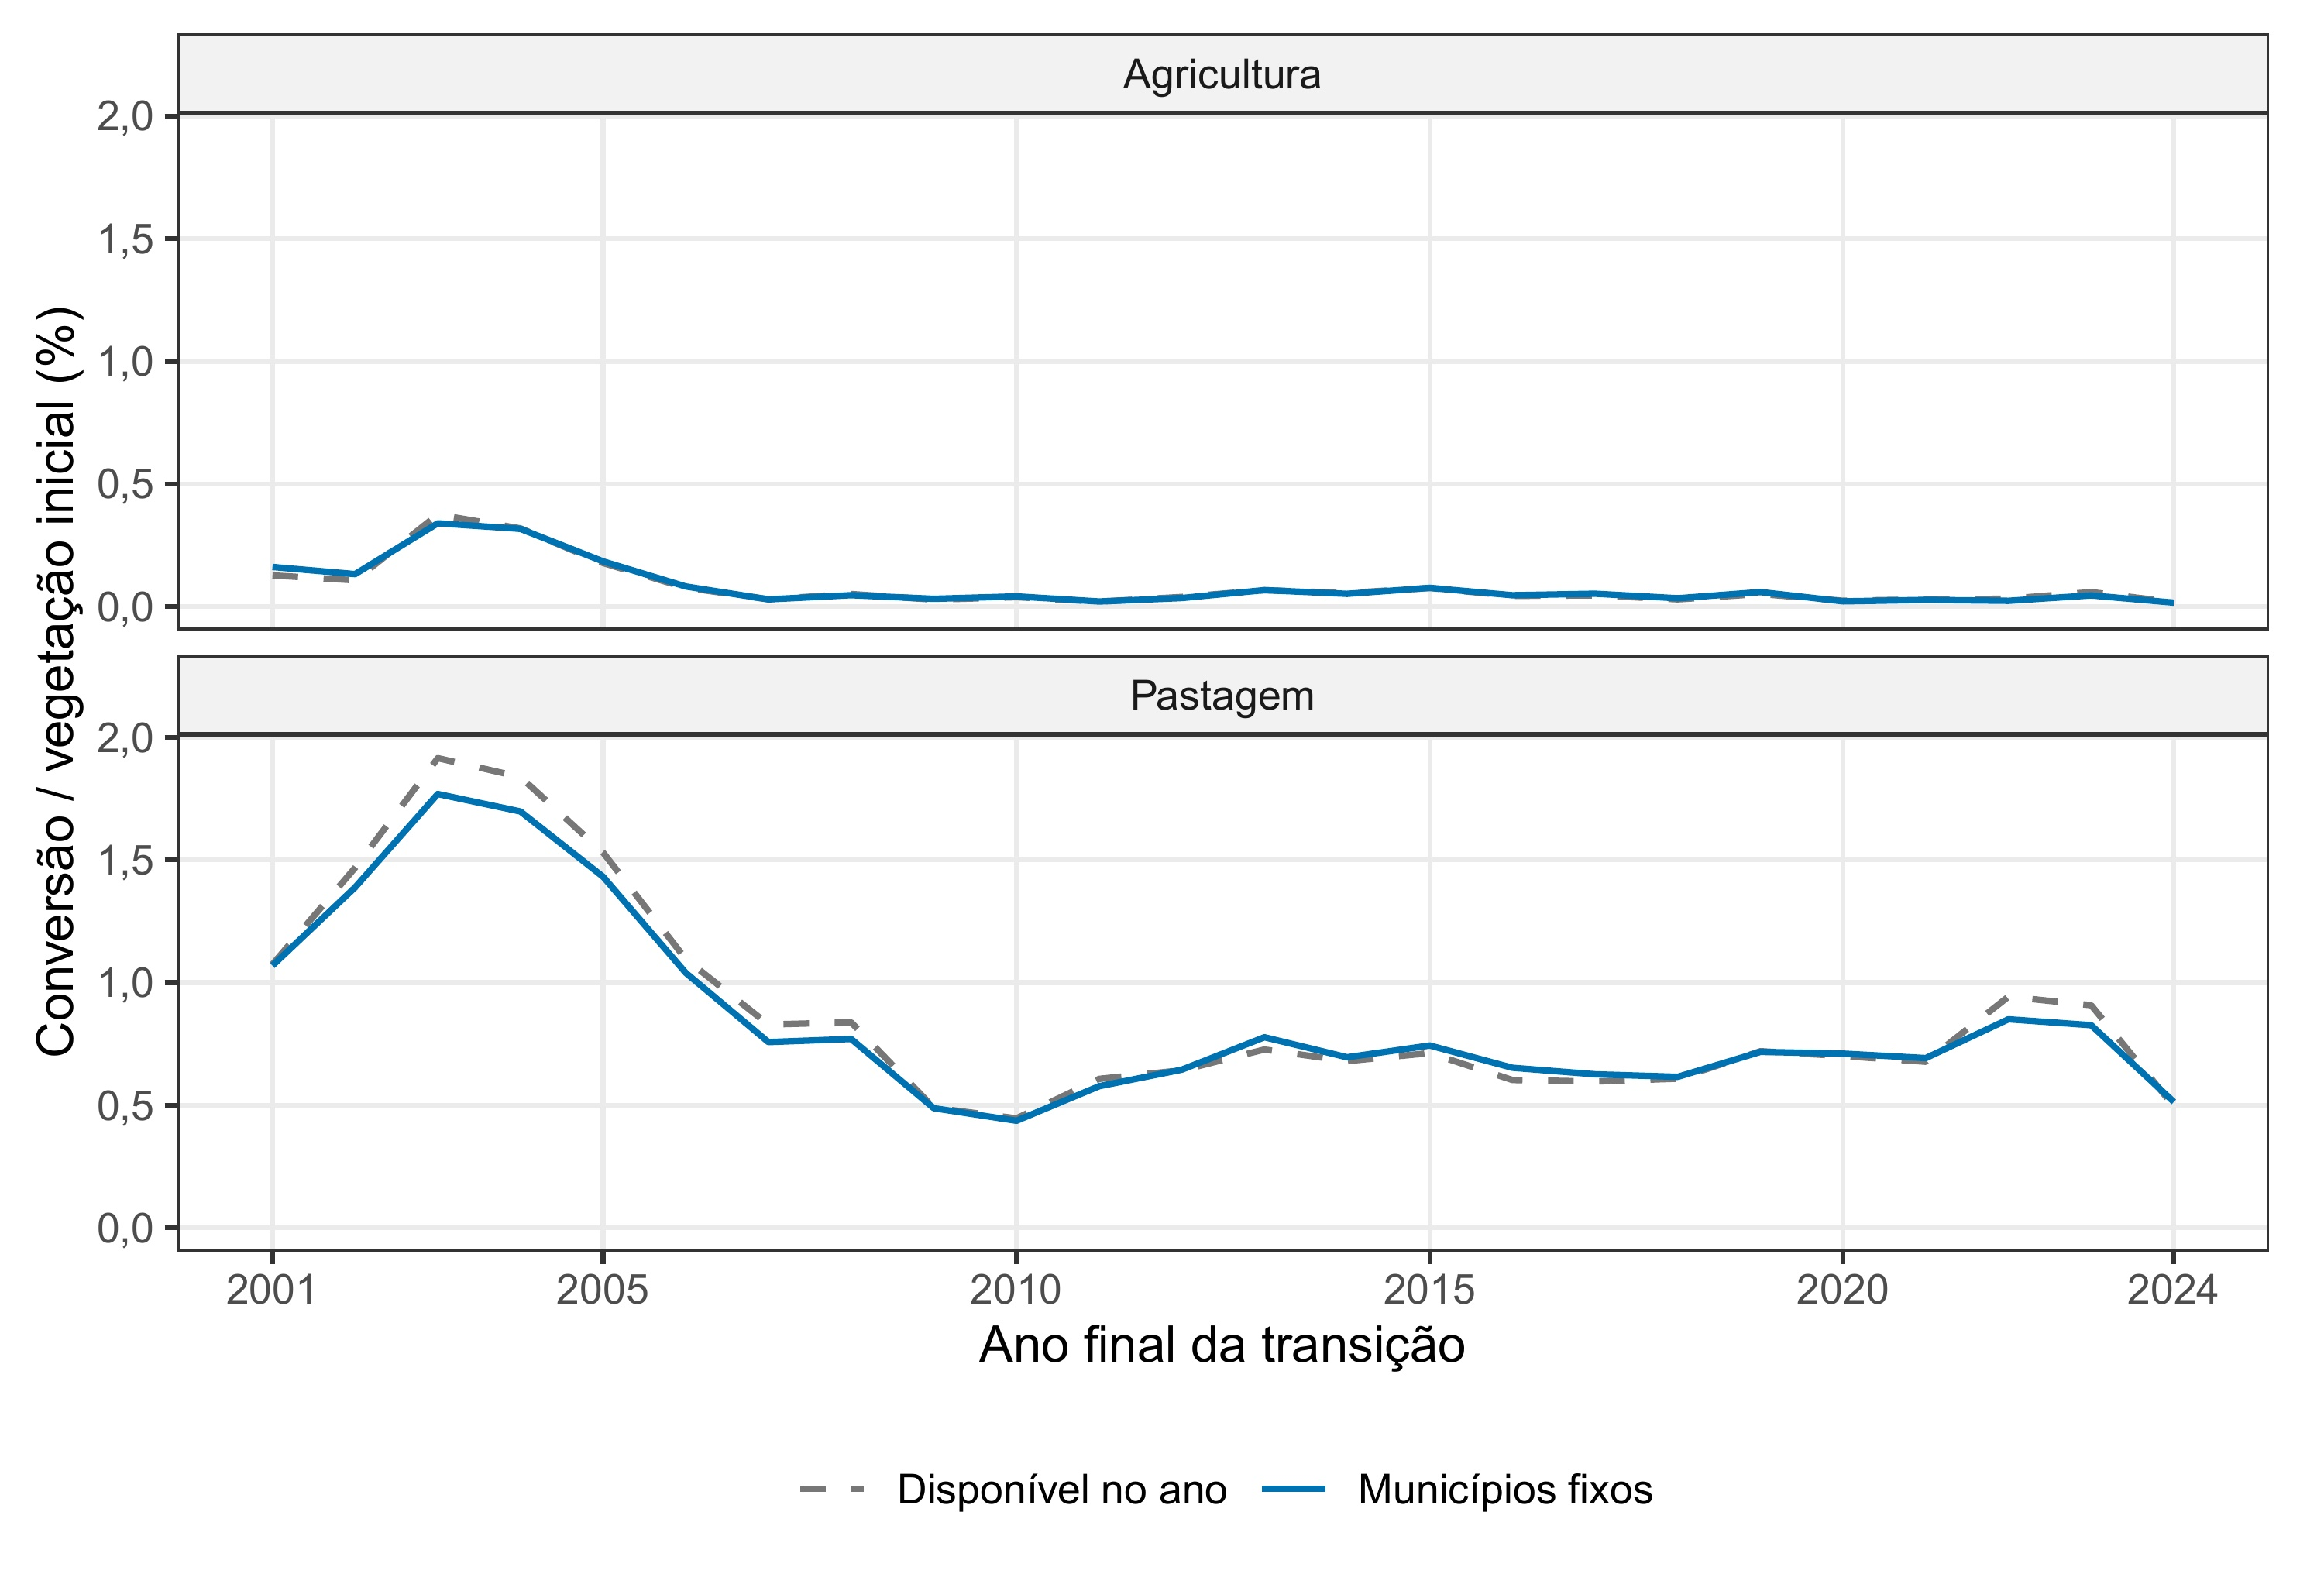
\includegraphics[width=\textwidth]{figuras/figura1.jpg}
\caption{Conversão bruta da vegetação nativa para agricultura e pastagem, 2001--2024}
\label{fig:h1-conversao}
\begin{minipage}{\textwidth}\normalsize\centering
Fonte: elaboração própria com MapBiomas 10.1 e malha IBGE 2023.
\end{minipage}
\end{figure}


Os preços internacionais de soja, milho e carne bovina provêm da \textit{Pink Sheet}. As cotações mensais foram deflacionadas pelo índice de preços ao consumidor urbano dos Estados Unidos (CPI-U) para dólares de poder de compra médio de 2024, exigindo doze meses para cada média anual \cite{WorldBank2026,BLSCPI2026}. A Figura~\ref{fig:h1-precos} apresenta índices com base 100 em 2000, permitindo comparar variações proporcionais entre produtos cotados em unidades diferentes. Os preços de 2000--2023 antecedem as conversões de 2001--2024. Em 2023, as três cotações reais superavam as de 2000, embora as taxas de conversão fossem menores nos extremos correspondentes. Essa comparação descritiva reúne mudanças de contexto e não identifica a resposta condicionada aos preços.

O contraste entre esses extremos não contradiz, por si, a associação mais positiva prevista em H1a: a hipótese compara a resposta entre capacidades locais, mantidas as demais condições, enquanto as séries agregadas reúnem mudanças produtivas, institucionais e de composição. A cotação da carne situa ainda uma alternativa de uso da terra, em diálogo com o problema de preços relativos examinado por \citeonline{Braganca2018}. Sua presença no gráfico contextualiza a comparação, sem transformar as três séries em medidas de rentabilidade ou de retorno recebido pelos produtores mato-grossenses.

\begin{figure}[H]
\centering
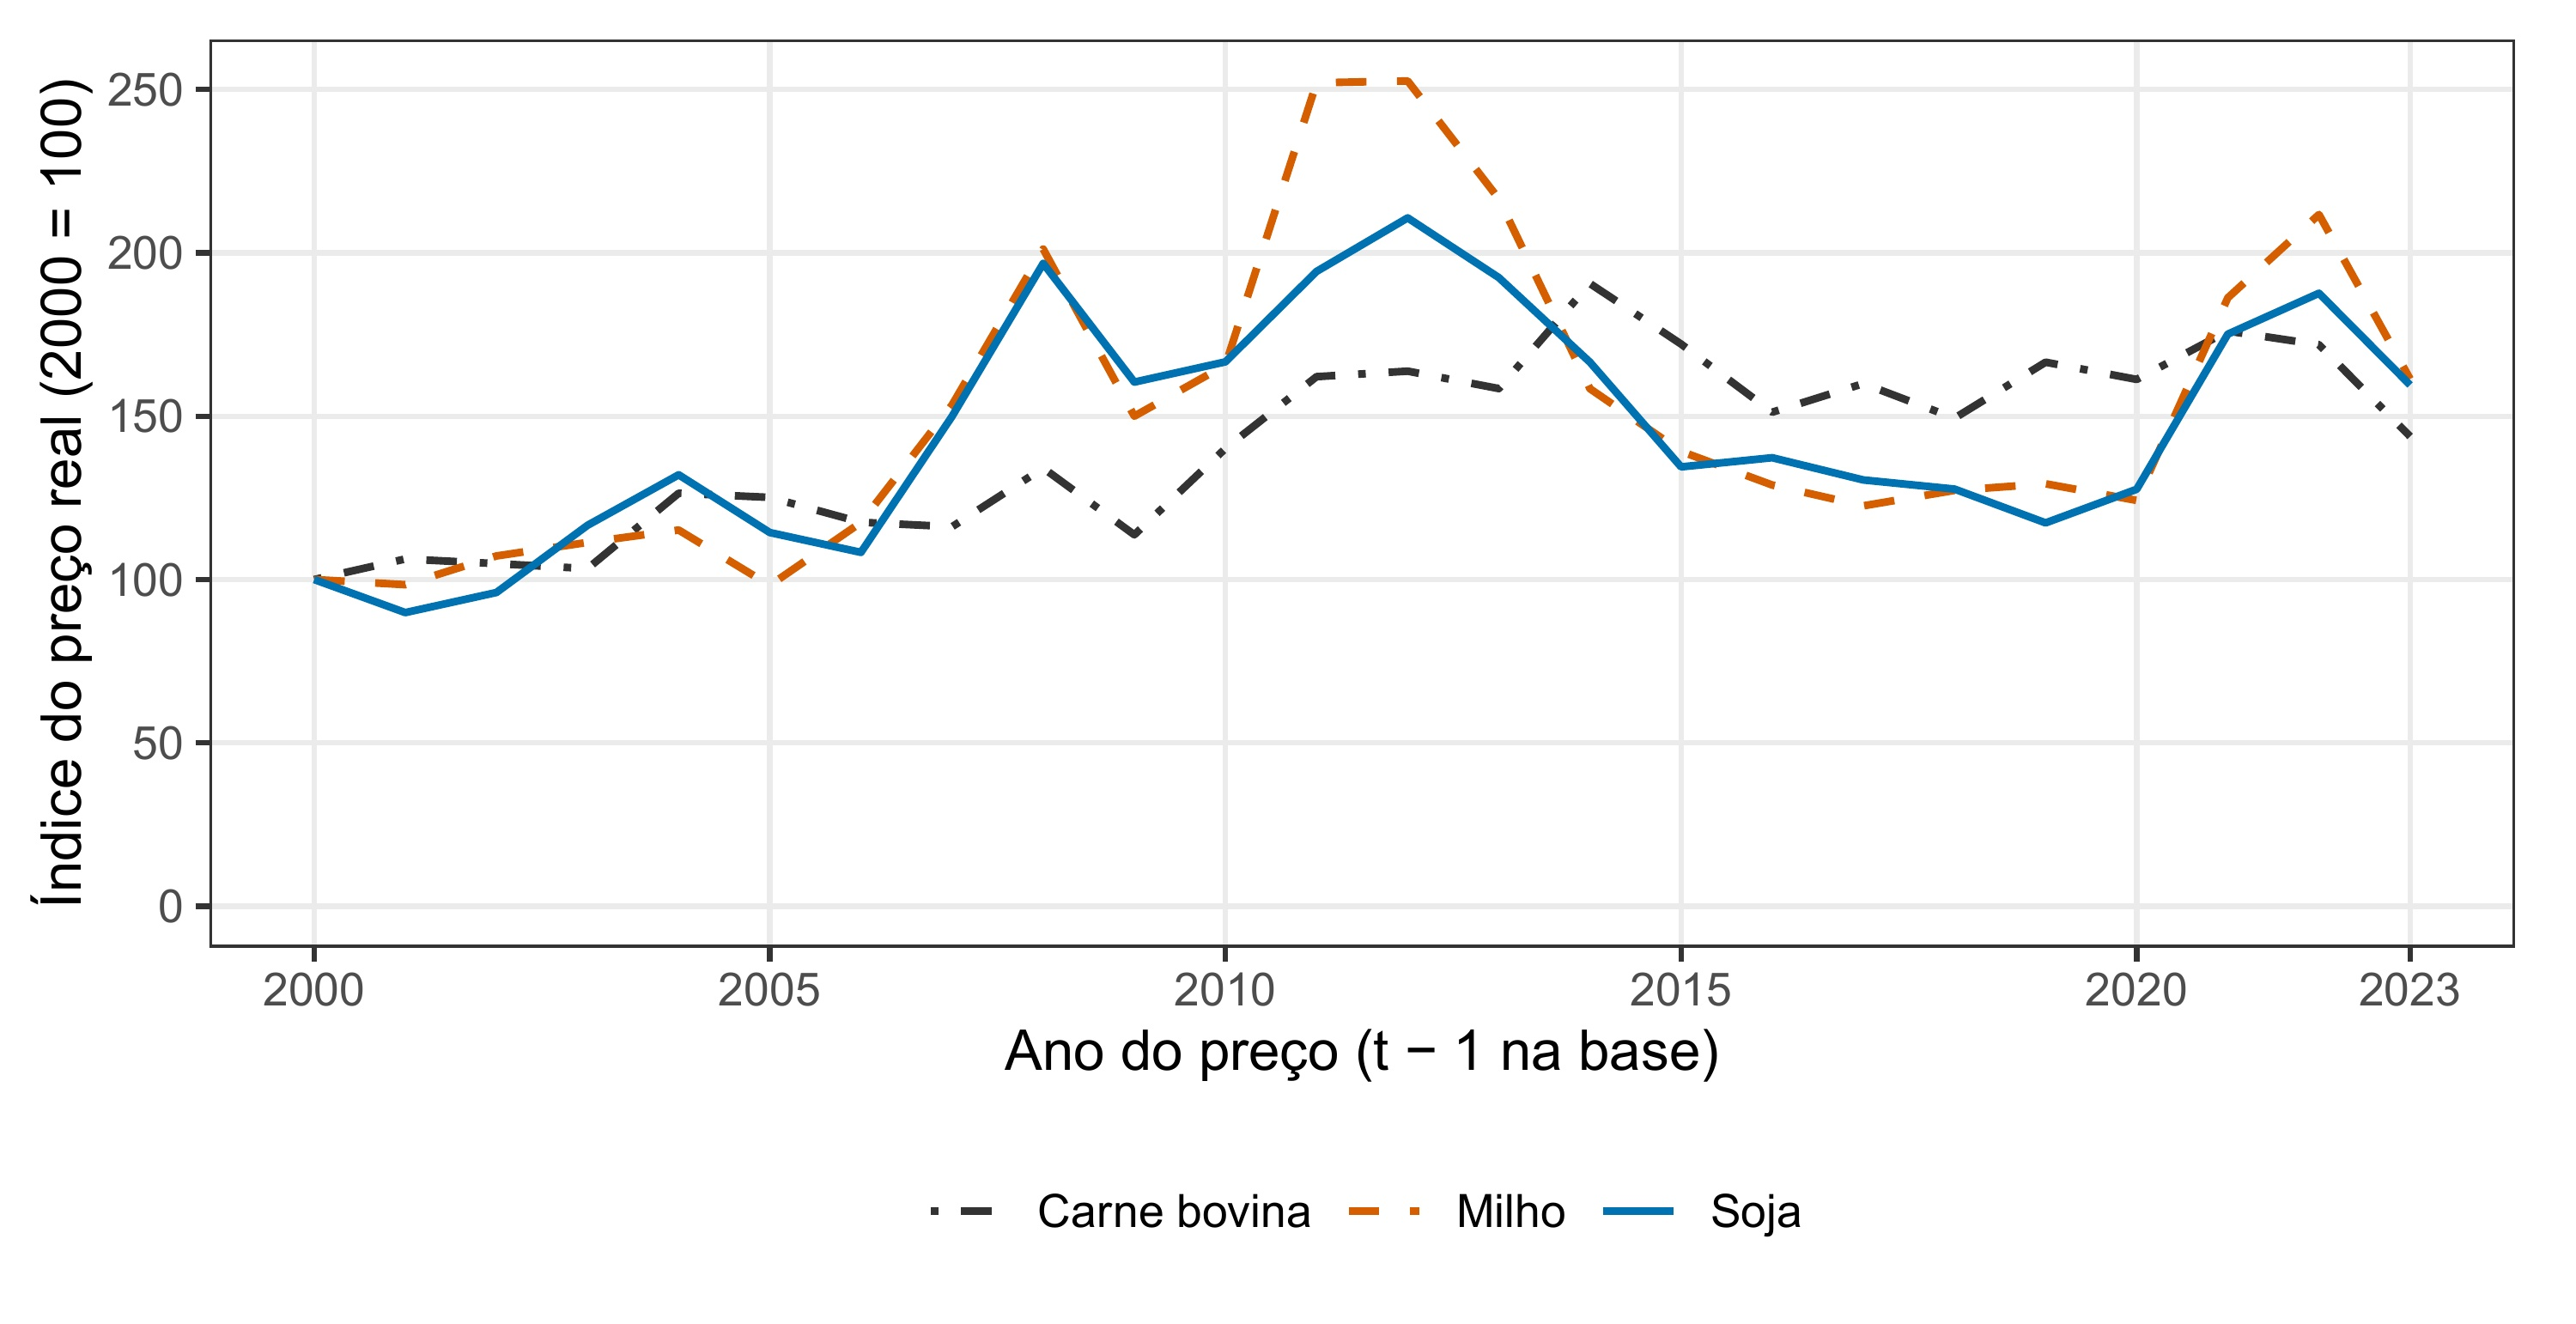
\includegraphics[width=\textwidth]{figuras/figura2.jpg}
\caption{Preços reais internacionais de soja, milho e carne bovina}
\label{fig:h1-precos}
\begin{minipage}{\textwidth}\normalsize\centering
Fonte: elaboração própria com Banco Mundial e CPI-U BLS/FRED.
\end{minipage}
\end{figure}


O potencial agrícola é medido pelo Global Agro-Ecological Zones (GAEZ), versão 4 em sequeiro e alto insumo, em quilogramas de matéria seca por hectare \cite{FAOGAEZ2021}. O indicador da melhor classe de aptidão de cada célula foi agregado por média dos pixels válidos, ponderada pelo cosseno da latitude para aproximar suas áreas. A climatologia é 1961--1990, mas a versão incorpora bases territoriais de 2010. Portanto, o indicador fixo não garante anterioridade de todos os componentes às decisões do painel. Ele descreve possibilidades sob condições padronizadas, sem representar rendimento comercial observado, tecnologia efetivamente empregada ou potencial específico das parcelas nativas disponíveis. O mesmo potencial padronizado é conservado nas diferentes amostras.

Na Tabela~\ref{tab:h1-capacidade}, cada município participa uma única vez. As medianas de potencial para soja e milho são maiores no grupo de predominância Cerrado que no amazônico, mas os intervalos entre os percentis 25 e 75 se sobrepõem. A classificação por bioma, portanto, não substitui a variação produtiva municipal. É essa variação que permite comparar a associação com uma cotação comum entre localidades com possibilidades diferentes, conforme o argumento de H1a. A tabela caracteriza o potencial; não demonstra que os municípios de maior capacidade converteram mais vegetação.

\begin{table}[H]
\centering\normalsize
\setlength{\tabcolsep}{6pt}
\caption{Potencial produtivo municipal por cultura e bioma predominante}
\label{tab:h1-capacidade}
\begin{tabular}{llrrr}
\hline
Cultura & Bioma & Municípios & Mediana & P25--P75 \\
\hline
Soja & Amazônia & 76 & 2.701 & 2.557--2.852 \\
Soja & Cerrado & 61 & 3.261 & 2.817--3.390 \\
Soja & Pantanal & 4 & 3.421 & 3.386--3.457 \\
Milho & Amazônia & 76 & 3.002 & 2.862--3.264 \\
Milho & Cerrado & 61 & 3.320 & 2.797--3.572 \\
Milho & Pantanal & 4 & 6.790 & 6.321--6.933 \\
\hline
\end{tabular}
\par\smallskip\begin{minipage}{\textwidth}\normalsize\centering
Fonte: elaboração própria com FAO/IIASA, GAEZ v4, e IBGE.
\end{minipage}
\end{table}


Os quatro municípios de predominância Pantanal apresentam potencial calculado elevado, especialmente para milho. Esse resultado exige distinguir a média dos pixels válidos no cenário GAEZ da viabilidade do cultivo nas parcelas disponíveis. Como discutido na fundamentação, condições de inundação, usos pecuários e acesso podem limitar a realização do potencial. Tampouco os quatro municípios integram igualmente as amostras de perdas. A diferença entre possibilidade padronizada, cultivo observado e informação suficiente para estimar o modelo impede interpretar a posição desse grupo como recomendação de expansão agrícola no bioma.

O desempenho anterior acrescenta uma dimensão distinta. A produção por hectare plantado reúne o rendimento colhido e a proporção da área plantada que chegou à colheita. Na Figura~\ref{fig:h1b-perdas}, as colunas correspondem a soja e milho, e o eixo horizontal registra a safra anterior. Os painéis superiores dividem a produção total pelas áreas plantada ou colhida dos mesmos municípios elegíveis, enquanto a referência é a média das previsões locais ponderada pela área plantada corrente. Nos painéis intermediários, as perdas médias atribuem igual peso aos municípios, e a frequência divide os casos de déficit de pelo menos 20\% pelo número elegível, mostrado abaixo. A média municipal não é a distância entre as curvas agregadas nem a fração da produção estadual perdida.

\begin{figure}[H]
\centering
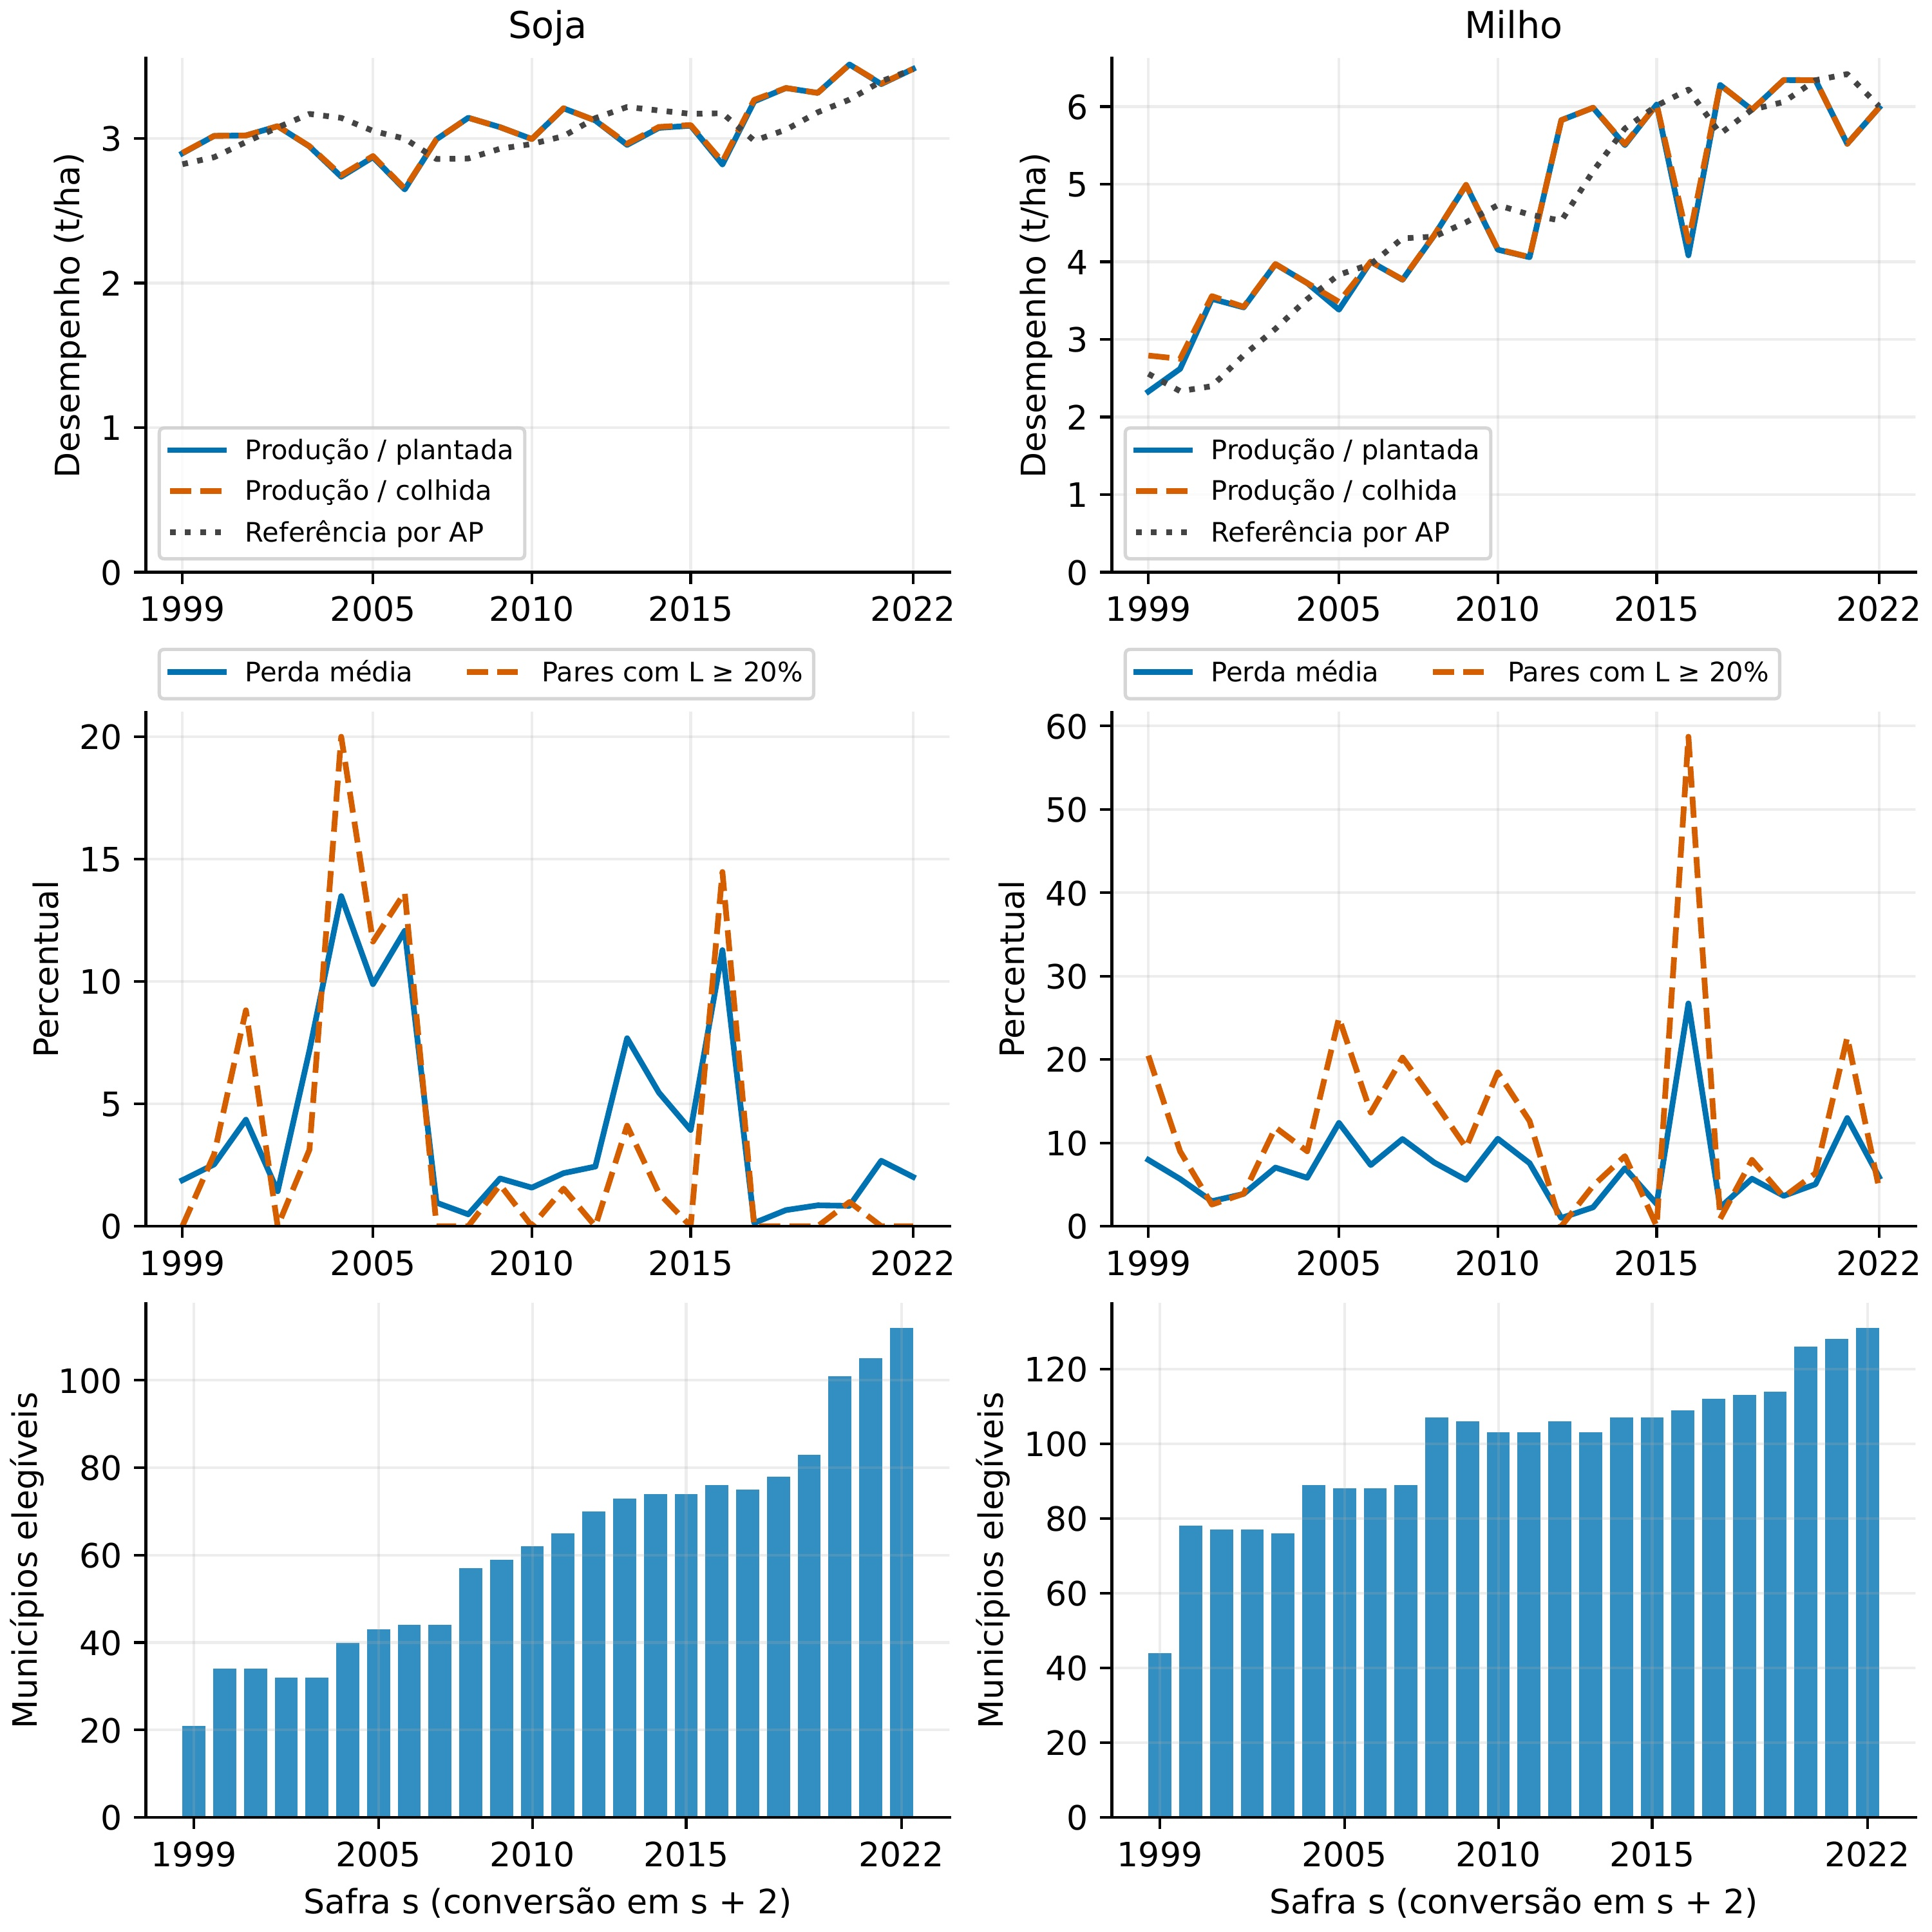
\includegraphics[width=\textwidth]{figuras/figura3.jpg}
\caption{Desempenho agrícola, perdas anteriores e cobertura das amostras ($AP$: área plantada; $L$: intensidade da perda; $s$: safra anual)}
\label{fig:h1b-perdas}
\begin{minipage}{\textwidth}\normalsize\centering
Fonte: elaboração própria com IBGE/PAM e MapBiomas 10.1.
\end{minipage}
\end{figure}


Em 2016, por exemplo, a amostra de milho apresentou 4,08 t/ha plantado e 4,26 t/ha colhido, diante de referência ponderada de 6,22 t/ha. A perda municipal média foi 26,7\%, e 58,7\% dos 109 municípios elegíveis registraram déficit de pelo menos 20\%. A comparação reúne menor desempenho nas áreas colhidas e não colheita de parte da área plantada, sem identificar a causa. No alinhamento principal, essa safra é vinculada ao preço de 2017 e à conversão entre 2017 e 2018. Essa sequência permite perguntar se uma perda anterior acompanha uma associação diferente com o preço subsequente, mas não mede a disponibilidade de recursos nem uma intenção de recuperar a produção por abertura. A cobertura muda entre safras; suas médias não descrevem a evolução do risco em um grupo fixo.

A disponibilidade de histórico também difere entre culturas e territórios. Antes da remoção dos grupos unitários dos efeitos fixos, as perdas válidas da soja cobrem 43,0\% dos pares com conversão observada no grupo amazônico e 63,7\% no Cerrado. No milho, essas proporções são próximas de 86\% nos dois grupos. No Pantanal, há 28 pares elegíveis de soja em dois municípios e 52 de milho em três, número que se reduz na estimação. Em todo o estado, a amostra elegível reúne 42 ocorrências de perda de pelo menos 20\% na soja e 283 no milho. Esses números descrevem o suporte de H1b, não uma comparação de risco entre culturas ou biomas: cultivo, registro e composição diferem, e os pares observados não constituem choques de preço independentes.

Na Tabela~\ref{tab:h1b-composicao}, as médias e medianas atribuem o mesmo peso a cada par município--ano. A coluna observada reúne os 2.772 pares de conversão; soja e milho são subconjuntos sobrepostos com perda anterior válida. As taxas usam o estoque nativo inicial, e os potenciais fixos reaparecem em cada ano observado. A conversão agrícola média é menor nos subconjuntos elegíveis, sobretudo no milho. A tabela antecipa, assim, que incluir perdas modifica também a composição da amostra. A chuva caracteriza outra condição variável no tempo: sua anomalia anual, em milímetros, compara a precipitação com a média municipal de 1981--2000, utilizando a série Climate Hazards Group InfraRed Precipitation with Station data (CHIRPS). Ela não corresponde diretamente ao clima da safra anterior.

\begin{table}[H]
\centering\normalsize\captionstyle{\centering}\normalcaption
\caption{Composição da amostra observada e das amostras com perdas anteriores}\label{tab:h1b-composicao}
\begin{tabular}{p{5.2cm}*{3}{p{3.3cm}}}
\hline
Indicador & Observada & Soja & Milho \\
\hline
Pares município--ano & 2.772 & 1.488 & 2.381 \\
Municípios & 137 & 115 & 137 \\
Conversão agrícola (\%) & 0,112 (0,014) & 0,106 (0,029) & 0,085 (0,013) \\
Conversão para pastagem (\%) & 1,192 (0,799) & 0,943 (0,701) & 1,142 (0,765) \\
Potencial da soja (kg MS/ha) & 2.942 (2.837) & 2.981 (2.950) & 2.965 (2.916) \\
Potencial do milho (kg MS/ha) & 3.245 (3.135) & 3.177 (3.066) & 3.269 (3.144) \\
Anomalia de chuva em t (mm) & -31,4 (-36,4) & -33,3 (-43,7) & -33,3 (-41,2) \\
\hline
\end{tabular}
\par\smallskip\begin{minipage}{\textwidth}\normalsize\centering
Fonte: elaboração própria com MapBiomas, IBGE/PAM, GAEZ v4 e CHIRPS.
\par\medskip
\raggedright Legenda: Médias, com medianas entre parênteses, com igual peso aos pares município--ano. MS: matéria seca. As amostras das culturas se sobrepõem; elegibilidade antecede a remoção de grupos unitários dos efeitos fixos.
\end{minipage}
\end{table}


A seleção pelo histórico conecta a descritiva à interpretação dos resultados. Uma alteração no gradiente preço×capacidade pode decorrer da entrada em uma amostra com menor conversão média, mesmo antes de incluir a perda no modelo. Por isso, a estratégia seguinte compara a especificação sem perdas na amostra original e na amostra comum, para somente então acrescentar os termos de H1b. As diferenças descritivas orientam essa comparação, sem determinar antecipadamente o sinal dos coeficientes.
